\documentclass[a4paper,12pt]{article}

\usepackage[english]{babel}
\usepackage[utf8]{inputenc}
\usepackage[T1]{fontenc}

% Margini e Layout
\usepackage[a4paper,top=2cm,bottom=2cm,left=2cm,right=2cm]{geometry}
\linespread{1.1}

% Pacchetti Standard
\usepackage{csquotes}
\usepackage{amsmath} 
\usepackage{amssymb}
\usepackage{graphicx}
\usepackage{subcaption}
\usepackage{siunitx}
\usepackage{pdfpages} % Per inserire i PDF

% --- TIKZ & PGFPLOTS ---
\usepackage{tikz}
\usetikzlibrary{positioning}
\usepackage{pgfplots}
\pgfplotsset{compat=1.18}

% --- BIBLIOGRAFIA ---
\usepackage[style=numeric,sorting=none]{biblatex}
\addbibresource{Sections/bibliography.bib}

% --- HYPERREF (Per indice cliccabile e link) ---
\usepackage{xcolor}
\usepackage[
    colorlinks=true,
    linkcolor=blue,            
    citecolor=red!70!black,    
    urlcolor=cyan,             
    bookmarks=true,
    bookmarksopen=true,        % Apre i segnalibri nel visualizzatore PDF
    pdftitle={DHM Project},            
]{hyperref}

% Attiva la numerazione (necessaria per l'indice)
\pagenumbering{arabic} 

\begin{document}

% --- INTESTAZIONE ---
\begin{center}
    \begin{minipage}{0.09\textwidth}
        
\includegraphics[width=\linewidth]{logo.png} 
    \end{minipage}
    \hfill
    \begin{minipage}{0.85\textwidth}
        \vspace{-0.01cm} 
        {\large \textbf{LABORATORY OF BIOPHOTONICS II A.A.2025-2026}}
         \vspace{0.2cm} 
      \hspace*{2.5cm}{ \textit{Giuseppe Occhialini Department Of Physics}}
    \end{minipage}
\end{center}
\vspace{1cm}

% --- TITOLO ---
\begin{center}
    {\Huge \textbf{DHM}}\\[0.6cm]
    {\large C. Catanoso, A. Lavecchia, F. Bellina, G. Marzorati}
\end{center}
\vspace{1cm}

% --- INDICE ---
\tableofcontents
\newpage

% --- INSERIMENTO SEZIONI ---
\section{Introduction}

Digital holographic microscopes (DHMs) have been widely applied in material and biological
applications. For instance, among many biological and biomedical applications, DHM
systems are used for analyzing cells and tissues, as well as disease diagnosis and screening
 and assessing the polarimetric properties of biomedical samples.
The performance of DHM technologies relies heavily on computational reconstruction processing to provide trustworthy
sample information. The required computational reconstruction algorithms are uniquely
dependent on the optical configuration of the DHM system. An incorrect selection of the
reconstruction algorithms leads to distorted and inaccurate amplitude and phase measurements. 

DHM systems record the interference pattern (e.g., hologram) generated between the scattered light from the sample, named object wavefront, and a known reference wavefront.
DHM systems operate in off-axis, slightly off-axis, or in-line (also known as on-axis) configurations based on the interference angle.
Therefore, the selection of the DHM reconstruction
algorithms depends on this interference angle. 

For example, off-axis DHM systems enable the
reconstruction of the complex amplitude distribution of an object wavefront from a single hologram since the three components of the hologram are entirely separable in the Fourier
domain.

Therefore, the reconstruction algorithm in off-axis DHM systems requires the spatial filtering of the sample frequencies from the hologram’s spectrum. In contrast, the
spectral components of a hologram in the Fourier domain overlay totally or partially in in-line
and slightly off-axis DHM systems, respectively, requiring the acquisition of multiple phase-shifted holograms and the application of phase-shifting (PS) techniques [1, 26] to reconstruct the desired object information. 

In addition, the selection of the DHM reconstruction algo-
rithms also depends on whether the DHM imaging system operates in telecentric or non-telecentric regimes.
 DHM systems operating in the telecentric regime only require the interference angle compensation in the off-axis and slightly off-axis configuration.
Oppositely, non-telecentric DHM systems should compensate for the spherical phase factor recognized in
DHM and associated with a non-telecentric imaging system. Finally, the DHM configuration can operate in an image-plane configuration, meaning that in-focus DHM holograms
are recorded, so there is no need to apply numerical propagations to focus the amplitude and
phase images. However, if out-of-focus holograms are recorded, the user should numerically
propagate the complex amplitude distribution to provide in-focus images. Among the different
numerical propagation algorithms to reconstruct DHM images, the most used computational
approaches in DHM are the angular spectrum for short propagation distances [31, 32] and the
Fresnel transform algorithm for large propagation distances [33].
Still, each research group within the DHM community develops and implements its own
computational reconstruction algorithms based on its experimental digital holography (DH)
and DHM systems. Nonetheless, some research groups have developed and implemented
libraries and plugins to address the need for an open-source reconstruction toolbox in DHM
and DH. The main difference between DHM and DH systems is the utilization of a micro-
scopic imaging system in the object wave. 

\subsubsection{Background: Reconstruction algorithms for different optical
DHM configurations}

DHM systems are based on optical interferometry, which involves the digital recording of the
interference pattern (e.g., digital hologram) between the complex amplitude distribution scat-
tered by a microscopic object (e.g., the object wavefront) and a uniform reference wavefront.
DHM systems are colloquially known as hybrid imaging systems since the final reconstructed
amplitude or phase images are obtained after further computational processing of the digital
hologram. This second stage, known as the reconstruction stage, depends on the optical con-
figuration of the DHM system. This section thoroughly describes different DHM configura-
tions and their corresponding numerical reconstruction algorithms.
For simplicity, WE? have chosen a traditional DHM setup based on a Mach-Zehnder interfer-
ometer operating in transmission mode, see Fig 1(A) METTERE FIGURA. The light generated from a laser of wave-length λ is collimated by a converging lens (CL) and the resultant plane wavefront impinges a
cubic beam splitter (BS1) to generate the object (O) and the reference (R) wavefronts. A micro-
scopic imaging system is inserted in the object arm of the DHM system. This microscopic
imaging system comprises an infinity-corrected microscopic objective (MO) lens and a tube
lens (TL) which forms an image of the wavefront scattered by the microscopic sample with
amplitude distribution o(x,y). If the object is set at the front-focal plane (FFP) of the MO lens,
the image of the sample whose amplitude distribution is uIP (x,y) is then obtained at the back-
focal plane (BFP) of the TL. This plane is known as the microscope’s image plane (IP) [mettere e discutere eventualemente la formula (1)]. #fare il cammino ottico meglio

The hologram, captured at any plane from the IP, is the result of the interference between
the complex wavefield produced by the microscope at a distance zfrom the IP,....
discutere la formula (2) e (3) 
 The irradiance distribution of the hologram h(x,y;z) is ... (4)

On the other hand, the third
and fourth terms in Eq (4) encode the complex amplitude information of the object wavefront
scattered by the sample. These terms represent the object’s real and twin images. From Eq (4),
it is clear that the object information o(x,y), encoded in u(x,y;z) is mixed with other undesired
terms. The reconstruction algorithms aim to separate these undesired terms from the object
information to provide well-contrast amplitude and phase images from the complex in-focus
amplitude distribution uIP (x,y) = u(x,y;z= 0) with minimum distortions. Assuming that the
reference wavefront is plane, the 2D Fourier transform of the hologram H(u,v;z) is ....

% ============================================================
\section{Introduzione e motivazione}
% ============================================================

L'imaging non invasivo di cellule biologiche viventi nel loro ambiente naturale è un
problema centrale nella biofisica moderna. Le tecniche di microscopia classica a
contrasto di fase (Zernike) o a contrasto di interferenza differenziale (Nomarski) sono
strumenti preziosi per rendere visibili campioni trasparenti e non colorati, ma offrono
soltanto informazioni qualitative: non è possibile, con esse, ricavare in modo assoluto
il ritardo di fase prodotto dal campione.
% ? sistemare questa parte su in base al campione dato
% * riscrivere le parole in italiano tecnice, in inglese

Le tecniche interferometriche digitali superano questo limite fornendo una misura
\emph{quantitativa} dello sfasamento del fronte d'onda trasmesso attraverso il
campione. In particolare, la \textbf{Microscopia Olografica Digitale} (DHM,
\textit{Digital Holographic Microscopy}) consente di ricostruire numericamente, a
partire da un singolo ologramma registrato da una camera CCD, sia l'immagine di
ampiezza che quella di \emph{contrasto di fase quantitativo} con risoluzione
interferometrica, senza l'impiego di agenti di contrasto.

Il vantaggio fondamentale è che la DHM fornisce una mappa spaziale del
\textbf{cammino ottico} (OPL, \textit{Optical Path Length}) punto per punto nel piano
del campione. Come si vedrà, tale grandezza dipende in modo \emph{accoppiato} da
due proprietà fisiche della cellula:
\begin{enumerate}
  \item lo \textbf{spessore locale} $h$ della cellula (morfometria), e
  \item l'\textbf{indice di rifrazione integrale} $\bar{n}_c$, ovvero la media
        dell'indice di rifrazione intracellulare lungo lo spessore.
\end{enumerate}

Misurare queste due quantità separatamente da un'unica immagine di fase è un
problema sottodeterminato. Questa relazione presenta, tra le altre cose, una procedura sperimentale
originale — la \textbf{procedura di disaccoppiamento} — che risolve tale
indeterminazione in modo elegante e rigoroso. % ? basato su articolo ...

% ============================================================
\section{Principio fisico: cammino ottico e sfasamento}
% ============================================================

\subsection{L'indice di rifrazione e la velocità della luce}

L'indice di rifrazione di un mezzo è definito come
\[
  n = \frac{c}{v},
\]
dove $c$ è la velocità della luce nel vuoto e $v$ è la velocità di fase nel mezzo.
%Materiali biologici come il citoplasma cellulare hanno indici di rifrazione
%superiori a quello del mezzo extracellulare acquoso ($n_m \approx 1.33$--$1.34$),
%risultando in un rallentamento della luce che attraversa la cellula rispetto a quella
%che viaggia nel mezzo circostante.
Materiali o soluzioni che simulano il citoplasma cellulare hanno indici di rifrazione
superiori a quello del mezzo extracellulare acquoso ($n_m \approx 1.33$--$1.34$) (dato in questa anologia dal campione sintetico di nastro adesivo)
risultando in un rallentamento della luce che attraversa il campione rispetto a quella
che viaggia nel mezzo circostante.

\subsection{Definizione del cammino ottico}

Sia $z$ la coordinata assiale (lungo l'asse ottico del microscopio). Il
\textbf{cammino ottico} $\mathrm{OPL}$ di un raggio che percorre un mezzo
\textit{stratificato} di spessore totale $D$ è
\[
  \mathrm{OPL} = \int_0^D n(z)\,dz,
\]
dove $n(z)$ è il profilo dell'indice di rifrazione lungo $z$.

\subsection{Configurazione sperimentale della DHM}

Il campione (un multistrato di layer di nastro adesivo) è posto in una camera di perfusione (alloggiamento circolare apposito) di
altezza $D$ riempita di soluzione con indice di rifrazione $n_m$ uniforme e costante (SOLUZIONE DI SACCAROSO A PERCENTUALE, CON UN n MISURATO).
Il campione occupa localmente una regione di spessore $h_i$ (per ciascun pixel $i$
dell'immagine), con \textbf{indice di rifrazione interno} al campione $n_{c,i}(z)$ variabile in senso
assiale.

Il cammino ottico per il pixel $i$ è:
\begin{equation}
  \mathrm{OPL}_i
  = \int_0^{h_i} n_{c,i}(z)\,dz + n_m(D - h_i)
  = \left(\bar{n}_{c,i} - n_m\right)h_i + n_m D,
  \label{eq:OPL}
\end{equation}
dove si è definito l'\textbf{indice di rifrazione integrale} come la media integrale:
\[
  \bar{n}_{c,i} = \frac{1}{h_i}\int_0^{h_i} n_{c,i}(z)\,dz.
\]

\subsection{Relazione tra OPL e fase misurata}

La fase $\varphi_i$ misurata dal DHM per il pixel $i$ è legata all'OPL dalla
relazione:
\[
  \mathrm{OPL}_i = \frac{\lambda}{2\pi}\,\varphi_i,
\]
dove $\lambda$ è la lunghezza d'onda del laser. Sostituendo~\eqref{eq:OPL}:
\begin{equation}
    \color{red}
  \varphi_i = \frac{2\pi}{\lambda}\left[\left(\bar{n}_{c,i} - n_m\right)h_i + n_m D\right].
  \label{eq:fase_completa}
\end{equation}

Il termine $n_m D$ è una costante di riferimento misurabile in zone prive di campione (o di cellule)
e viene sottratta sperimentalmente. Il segnale \emph{di fase} è quindi:
\begin{equation}
  \color{red}
  \varphi_i = \frac{2\pi}{\lambda}\left(\bar{n}_{c,i} - n_m\right)h_i.
  \label{eq:fase_cella}
\end{equation}

\paragraph{Il problema dell'accoppiamento.}
L'equazione~\eqref{eq:fase_cella} contiene \textbf{due incognite} per ciascun
pixel $i$: lo spessore $h_i$ e l'indice di rifrazione integrale
$\bar{n}_{c,i}$. Una singola misura di fase non è sufficiente a determinare
entrambe le quantità. Si noti in particolare che variazioni di $h_i$ e di
$\bar{n}_{c,i}$ possono produrre identiche variazioni di $\varphi_i$, rendendo
ambigua l'interpretazione del segnale di fase da sola.

% ============================================================
\section{Stabilità del sistema e prestazioni della DHM}
% ============================================================

Prima di illustrare la procedura di disaccoppiamento è importante quantificare le
prestazioni del sistema, poiché esse determinano la precisione finale delle misure.

\begin{itemize}
  \item \textbf{Stabilità temporale della fase:} mediando 16 immagini di fase
        consecutive, si ottiene una stabilità temporale equivalente a
        $\lambda/1800 \approx 0{,}2°$ per ciascun pixel.
  \item \textbf{Sensibilità verticale (assiale):} la stabilità di fase di $0{,}2°$
        corrisponde, per campioni con indice di rifrazione tipico
        $\bar{n}_c \approx 1{,}375$, a una sensibilità verticale di circa
        \textbf{11 nm}.
  \item \textbf{Risoluzione laterale:} limitata dalla diffrazione,
        $\approx 0{,}6\ \mu\mathrm{m}$ per un obiettivo con
        $\mathrm{NA} = 0{,}8$ a $\lambda = 658\ \mathrm{nm}$ (criterio di
        Rayleigh per illuminazione coerente).
  \item \textbf{Tempo di acquisizione:} limitato dal tempo di esposizione della
        camera ($\sim 20\ \mu\mathrm{s}$), con ricostruzione in tempo reale a
        più di 10 immagini/s.
  \item \textbf{Bassa intensità di illuminazione:} l'irradianza sul campione è
        $\sim 200\ \mu\mathrm{W/cm^2}$, svariati ordini di grandezza inferiore a
        quella tipica della microscopia confocale a scansione laser.
\end{itemize}

% ============================================================
\section{La procedura di disaccoppiamento}
\label{sec:decoupling}
% ============================================================

\subsection{Idea fondamentale}

Per risolvere l'indeterminazione dell'equazione~\eqref{eq:fase_cella}, si introduce
una \emph{seconda misura di fase indipendente} sullo \emph{stesso campione},
ottenuta modificando in modo controllato e noto l'indice di rifrazione del mezzo
extracellulare (mezzo fuori dal campione). In questo modo si ottiene un \textbf{sistema di due equazioni in due
incognite} ($h_i$ e $\bar{n}_{c,i}$) che può essere risolto analiticamente.

\subsection{Protocollo sperimentale}

La procedura prevede la perfusione sequenziale di \textbf{due soluzioni}:

\begin{enumerate}
  \item \textbf{Soluzione standard}: mezzo extracellulare (acqua + saccarosio) con indice di rifrazione
        $n_m$ e osmolarità $\Pi_0$. Si registra l'ologramma e si ricostruisce la
        mappa di fase $\varphi_{1,i}$.

  \item \textbf{Soluzione di disaccoppiamento}: mezzo extracellulare con indice di
        rifrazione $n'_m = n_m + \delta n$. Si registra il secondo ologramma e si ottiene $\varphi_{2,i}$.
\end{enumerate}

Il requisito di \textit{isosmoticità} è cruciale: esso assicura che $h_i$ non cambi tra le
due misure, in modo che l'unica differenza tra $\varphi_{1,i}$ e $\varphi_{2,i}$
sia dovuta esclusivamente alla variazione $\delta n$ dell'indice del mezzo
extracellulare.

\paragraph{Come si ottiene $\delta n$:}
Si sostituisce una molecola idrofila osmotica (presente nella soluzione standard
come agente osmotico) con una quantità equimolare di una diversa molecola idrofila
avente \emph{maggiore polarizzabilità molare}. Poiché la concentrazione molare
totale rimane invariata, l'osmolarità è conservata, mentre l'indice di rifrazione
aumenta di $\delta n$ noto e misurabile.

\subsection{Il sistema di equazioni}

Con le convenzioni sopra introdotte, le due misure di fase sono:

\begin{align}
  \varphi_{1,i} &= \frac{2\pi}{\lambda}\left(\bar{n}_{c,i} - n_m\right)h_i,
  \label{eq:phi1} \\[6pt]
  \varphi_{2,i} &= \frac{2\pi}{\lambda}\left(\bar{n}_{c,i} - n_m - \delta n\right)h_i.
  \label{eq:phi2}
\end{align}

Sottraendo~\eqref{eq:phi2} da~\eqref{eq:phi1}:
\begin{equation}
  \varphi_{1,i} - \varphi_{2,i}
  = \frac{2\pi}{\lambda}\,\delta n\, h_i.
  \label{eq:differenza}
\end{equation}

\subsection{Derivazione della formula per lo spessore cellulare}
\label{subsec:spessore}

Dall'equazione~\eqref{eq:differenza} si ricava immediatamente lo spessore:

\begin{equation}
  \boxed{
    h_i = \frac{\lambda}{2\pi}\,\frac{\varphi_{1,i} - \varphi_{2,i}}{\delta n}
  }
  \label{eq:spessore}
\end{equation}

\paragraph{Interpretazione.} Lo spessore $h_i$ è determinato dalla
\emph{differenza} tra i due segnali di fase, normalizzata per la variazione
$\delta n$ introdotta nella soluzione. È notevole il fatto che il risultato non
dipenda dall'indice di rifrazione intracellulare $\bar{n}_{c,i}$, che è
sconosciuto: il contributo di quest'ultimo si cancella nella differenza
$\varphi_{1,i} - \varphi_{2,i}$. Ciò rende la misura di $h_i$ \emph{intrinsecamente
robusta} rispetto all'eterogeneità dell'intracellulare.

Notiamo anche la consistenza dimensionale: $[\lambda/(2\pi)]$ ha le dimensioni di
una lunghezza, $[\delta n]$ è adimensionale (variazione dell'indice), e
$[\varphi_{1,i} - \varphi_{2,i}]$ è in radianti (adimensionale), quindi $[h_i]$
risulta correttamente una lunghezza.

\subsection{Derivazione della formula per l'indice di rifrazione integrale}
\label{subsec:indice}

Per ricavare $\bar{n}_{c,i}$, si sostituisce~\eqref{eq:spessore}
in~\eqref{eq:phi1}:
\[
  \varphi_{1,i}
  = \frac{2\pi}{\lambda}\left(\bar{n}_{c,i} - n_m\right)
    \cdot \frac{\lambda}{2\pi}\,\frac{\varphi_{1,i} - \varphi_{2,i}}{\delta n}.
\]
Semplificando:
\[
  \varphi_{1,i}
  = \left(\bar{n}_{c,i} - n_m\right)
    \frac{\varphi_{1,i} - \varphi_{2,i}}{\delta n}.
\]
Risolvendo per $\bar{n}_{c,i}$:
\[
  \bar{n}_{c,i} - n_m
  = \frac{\delta n\,\varphi_{1,i}}{\varphi_{1,i} - \varphi_{2,i}},
\]
e quindi:
\begin{equation}
  \boxed{
    \bar{n}_{c,i}
    = \frac{\delta n\,\varphi_{1,i}}{\varphi_{1,i} - \varphi_{2,i}} + n_m
  }
  \label{eq:indice}
\end{equation}

\paragraph{Interpretazione.}
La formula~\eqref{eq:indice} mostra che l'indice di rifrazione integrale è
determinato dal \emph{rapporto} tra il segnale di fase nella prima misura
$\varphi_{1,i}$ e la differenza $\varphi_{1,i} - \varphi_{2,i}$, scalato per
$\delta n$ e traslato di $n_m$. Si noti che:
\begin{itemize}
  \item Se $\delta n \to 0$ il metodo perde di sensibilità (il denominatore va
        a zero); occorre quindi una perturbazione $\delta n$ sufficientemente
        grande da essere misurabile, ma non così grande da perturbare
        biologicamente la cellula.
  \item $\bar{n}_{c,i}$ non dipende dalla lunghezza d'onda $\lambda$ né da $D$,
        essendo questi parametri già stati eliminati nel passaggio dalla fase al
        segnale cellulare~\eqref{eq:fase_cella}.
  \item Il risultato è valido pixel per pixel: si ottiene quindi una
        \emph{mappa spaziale} dell'indice di rifrazione integrale, non solo un
        valore medio.
\end{itemize}

\subsection{Riepilogo del sistema: forma matriciale}
\label{subsec:matriciale}

Il sistema di equazioni~\eqref{eq:phi1}--\eqref{eq:phi2} può essere scritto in
forma matriciale per evidenzirne la struttura lineare. Poniamo
$x_i = \bar{n}_{c,i}\,h_i$ e $y_i = h_i$. Allora:
\[
\begin{pmatrix} \varphi_{1,i} \\ \varphi_{2,i} \end{pmatrix}
= \frac{2\pi}{\lambda}
\begin{pmatrix} 1 & -n_m \\ 1 & -(n_m+\delta n) \end{pmatrix}
\begin{pmatrix} x_i \\ y_i \end{pmatrix}.
\]
Il determinante della matrice dei coefficienti è:
\[
  \Delta = \frac{(2\pi)^2}{\lambda^2}
  \left[-(n_m+\delta n) + n_m\right]
  = -\frac{(2\pi)^2}{\lambda^2}\,\delta n \neq 0
  \quad \text{se } \delta n \neq 0.
\]
La non-singolarità del sistema è garantita dal fatto che $\delta n \neq 0$,
confermando che la procedura di disaccoppiamento è ben posta se e solo se le due
soluzioni hanno indice di rifrazione \emph{diverso}.

% ============================================================
\section{Precisione e limiti della procedura}
% ============================================================

\subsection{Stime teoriche di accuratezza per campioni fissi}

Data la stabilità di fase di $\sigma_\varphi \approx 0{,}2°$ per il sistema DHM
considerato, le accuratezze teoriche delle quantità ricostruite per un singolo pixel
sono:
\begin{align*}
  \sigma_{h_i} &\approx \frac{\lambda}{2\pi}\,\frac{\sqrt{2}\,\sigma_\varphi}{\delta n}
               \approx 100\ \mathrm{nm}, \\[4pt]
  \sigma_{\bar{n}_{c,i}} &\approx 0{,}0004.
\end{align*}

Queste accuratezze sono ottenibili solo su \textbf{campioni fissi}, poiché
richiedono che il campione rimanga perfettamente immobile tra le due acquisizioni.

\subsection{Effetti dei micro-movimenti su campioni viventi}

Per campioni \emph{viventi}, la cellula esegue spontaneamente micro-movimenti
durante il tempo di scambio della soluzione nel canale di perfusione (tipicamente
$\sim 30\ \mathrm{s}$). Tali movimenti inducono fluttuazioni temporali del segnale
di fase dell'ordine di $0{,}5$--$1{,}5°$ per pixel, peggiorando significativamente
le accuratezze puntuali.

\subsection{La media spaziale come rimedio}

Per compensare gli artefatti da micro-movimenti, si applica una \textbf{media
spaziale} dell'indice di rifrazione su tutta la superficie cellulare:
\[
  \bar{n}_c = \frac{1}{N_\mathrm{cell}}\sum_{i \in S_\mathrm{cell}} \bar{n}_{c,i}.
\]
La superficie cellulare $S_\mathrm{cell}$ viene determinata tramite un algoritmo di
rilevazione dei bordi basato su gradienti, seguito da una procedura di erosione che
rimuove i pixel periferici con basso rapporto segnale-rumore.

Questo indice mediato $\bar{n}_c$ presenta una stabilità temporale di $0{,}0003$
su intervalli di 30 secondi. Come prima approssimazione, si utilizza poi $\bar{n}_c$
(invece di $\bar{n}_{c,i}$ pixel per pixel) nella formula dello spessore~\eqref{eq:spessore},
riscritta come:
\[
  h_i \approx \frac{\lambda}{2\pi}\,\frac{\varphi_{1,i}}{\bar{n}_c - n_m}.
\]

\paragraph{Accuratezze pratiche su campioni viventi.}
Con la media spaziale:
\begin{itemize}
  \item Lo spessore locale $h_i$ ha un'accuratezza di $\sim 1\ \mu\mathrm{m}$.
  \item Mediando su $\sim 36$ pixel adiacenti, l'accuratezza locale migliora a
        $\sim 0{,}7\ \mu\mathrm{m}$.
  \item Lo spessore medio di una regione cellulare ha un'accuratezza di poche
        decine di nanometri.
  \item La variazione spaziale dell'indice integrale è stimata in $\sim 0{,}005$.
\end{itemize}

% ============================================================
\section{Discussione critica delle formule (4) e (5)}
% ============================================================

\subsection{Formula (4): misura dell'indice di rifrazione integrale}

\begin{equation*}
  \bar{n}_{c,i}
  = \frac{\delta n\,\varphi_{1,i}}{\varphi_{1,i} - \varphi_{2,i}} + n_m
  \tag{4}
\end{equation*}

\paragraph{Struttura matematica.}
Il termine $\dfrac{\varphi_{1,i}}{\varphi_{1,i} - \varphi_{2,i}}$ è un rapporto
di fasi. Poiché $\varphi_{2,i} < \varphi_{1,i}$ (la seconda soluzione ha indice
più alto, quindi lo sfasamento prodotto dalla cellula rispetto al mezzo è minore),
il denominatore è positivo e l'indice risultante è maggiore di $n_m$, come
fisicamente richiesto.

\paragraph{Dipendenza da $\delta n$.}
La sensibilità della misura aumenta con $\delta n$: una perturbazione maggiore
produce una differenza $\varphi_{1,i} - \varphi_{2,i}$ più grande, riducendo
l'errore relativo sul rapporto. Tuttavia, $\delta n$ non può essere arbitrariamente
grande perché la molecola utilizzata per modificare l'indice non deve
attraversare la membrana cellulare (la si sceglie idrofila e di alto peso
molecolare) e l'isosmoticità deve essere mantenuta.

\paragraph{Limite per $\delta n \to \varphi_{1,i}$ (caso limite).}
Se $\varphi_{2,i} \to 0$, ovvero la seconda soluzione ha indice di rifrazione
pari a $\bar{n}_{c,i}$ stesso (la cellula diventa invisibile in fase), si ottiene
$\bar{n}_{c,i} = \delta n + n_m = n'_m$, il che è coerente.

\subsection{Formula (5): misura dello spessore cellulare}

\begin{equation*}
  h_i
  = \frac{\lambda}{2\pi}\,\frac{\varphi_{1,i} - \varphi_{2,i}}{\delta n}
  = \frac{\lambda}{2\pi}\,\frac{\varphi_{1,i}}{\bar{n}_{c,i} - n_m}
  \tag{5}
\end{equation*}

\paragraph{Due forme equivalenti.}
La formula (5) è presentata in due forme equivalenti:
\begin{enumerate}
  \item La \textbf{forma operativa} (a sinistra): utilizza direttamente la
        differenza delle fasi misurate e $\delta n$ noto. Non richiede la
        conoscenza di $\bar{n}_{c,i}$.
  \item La \textbf{forma esplicita} (a destra): si ottiene sostituendo la
        definizione di $\bar{n}_{c,i}$ e mostra che $h_i$ è legato alla fase
        nella prima soluzione, normalizzata per il contrasto di indice
        $\bar{n}_{c,i} - n_m$.
\end{enumerate}

\paragraph{Robustezza rispetto all'indice intracellulare.}
La forma operativa della (5) mostra che lo spessore può essere misurato
\emph{senza conoscere a priori} l'indice di rifrazione intracellulare. Questo è
il punto di forza del metodo: la misura morfometrica è separata e indipendente
dalla misura dell'indice.

\paragraph{Consistenza con la fisica.}
Nella forma esplicita, l'espressione $\dfrac{\lambda}{2\pi}\dfrac{\varphi_{1,i}}
{\bar{n}_{c,i}-n_m}$ ha un'interpretazione fisica immediata: il numeratore
$\dfrac{\lambda}{2\pi}\varphi_{1,i}$ è il cammino ottico extra prodotto dalla
cellula rispetto al mezzo, mentre il denominatore $\bar{n}_{c,i} - n_m$ è
l'eccesso di indice di rifrazione; il loro rapporto fornisce direttamente
lo spessore fisico.

\subsection{Relazione tra le due formule}

Si noti che le formule (4) e (5) non sono indipendenti: derivano dalla risoluzione
dello stesso sistema lineare~\eqref{eq:phi1}--\eqref{eq:phi2}. La coerenza tra
le due può essere verificata sostituendo~\eqref{eq:spessore}
in~\eqref{eq:fase_cella} e recuperando~\eqref{eq:indice}. Il sistema è dunque
\emph{completo e non ridondante}: la misura di due fasi $(\varphi_{1,i},
\varphi_{2,i})$ con un $\delta n$ noto determina univocamente sia $h_i$ che
$\bar{n}_{c,i}$.

% ============================================================
\section{Stima del volume cellulare dalla morfometria}
% ============================================================

Una volta noti gli spessori $\{h_i\}$ per tutti i pixel all'interno della superficie
cellulare $S_\mathrm{cell}$, il volume cellulare può essere stimato come:
\[
  V_\mathrm{cell}
  \approx N_\mathrm{cell}\,\frac{S_\mathrm{pixel}}{M^2}\,\bar{h}_\mathrm{cell},
\]
dove $N_\mathrm{cell}$ è il numero di pixel nella superficie cellulare,
$S_\mathrm{pixel}$ è l'area di un singolo pixel nella camera CCD, $M$ è l'ingrandimento
del DHM, e $\bar{h}_\mathrm{cell} = \dfrac{1}{N_\mathrm{cell}}\displaystyle\sum_{i \in S_\mathrm{cell}} h_i$
è lo spessore medio della cellula.

% ============================================================
\section{Interpretazione fisica dell'indice di rifrazione integrale}
% ============================================================

L'indice di rifrazione integrale $\bar{n}_c$ è strettamente legato alla
\textbf{composizione biochimica} del citoplasma. Nell'approssimazione di
campo medio di Lorentz-Lorenz, l'indice di rifrazione di una miscela acquosa di
biomolecole aumenta linearmente con la concentrazione di materiale non acquoso
(proteine, ioni, lipidi, ecc.):
\[
  \bar{n}_c \approx n_{\mathrm{H_2O}} + \alpha_\mathrm{spec}\,C_\mathrm{protein},
\]
dove $\alpha_\mathrm{spec}$ è l'incremento specifico di rifrazione per unità di
concentrazione (tipicamente $\approx 0{,}185\ \mathrm{ml/g}$ per le proteine) e
$C_\mathrm{protein}$ è la concentrazione proteica intracellulare.

Pertanto, una \emph{diminuzione} di $\bar{n}_c$ segnala una \textbf{diluizione
intracellulare} (ad es.\ ingresso di acqua), mentre un \emph{aumento} segnala
un incremento di concentrazione di materiale disciolto.

% ============================================================
\section{Conclusioni}
% ============================================================

La procedura di disaccoppiamento descritta in questo articolo rappresenta una
soluzione elegante a un problema fondamentale nella microscopia di fase
quantitativa: \emph{come separare il contributo morfometrico (spessore) da quello
ottico (indice di rifrazione) nel segnale di fase}.

Il metodo si basa su due principi fisici semplici:
\begin{enumerate}
  \item La fase prodotta da una cellula dipende \emph{linearmente} sia da $h_i$
        che da $\bar{n}_{c,i}$ (equazione~\eqref{eq:fase_cella}).
  \item Modificando l'indice del mezzo extracellulare di una quantità nota
        $\delta n$ a volume cellulare costante, si ottiene un secondo vincolo
        lineare che rende il sistema determinato.
\end{enumerate}

Le formule chiave:
\begin{align*}
  \bar{n}_{c,i} &= \frac{\delta n\,\varphi_{1,i}}{\varphi_{1,i}-\varphi_{2,i}} + n_m,
  \tag{4} \\[6pt]
  h_i &= \frac{\lambda}{2\pi}\,\frac{\varphi_{1,i}-\varphi_{2,i}}{\delta n},
  \tag{5}
\end{align*}
sono entrambe derivabili in due passaggi algebrici elementari dalla differenza e
dal rapporto delle equazioni~\eqref{eq:phi1} e~\eqref{eq:phi2}.

Le prestazioni del DHM — stabilità di fase equivalente a $\lambda/1800$, risoluzione
laterale diffrattiva, tempo di acquisizione di $\sim 20\ \mu\mathrm{s}$, assenza di
agenti di contrasto — rendono questa tecnica particolarmente adatta allo studio
\emph{in tempo reale} della dinamica cellulare, con applicazioni che spaziano dalla
misurazione dello stress osmotico alla fisiopatologia cellulare, dalla biofisica delle
membrane alla valutazione farmacologica.

% ! ---------------------------------------------

% ================================================================
\section{Contesto e obiettivo dell'esperimento}
% ================================================================

Il presente documento descrive un esperimento di calibrazione e validazione della
procedura DHM, ispirato al metodo di disaccoppiamento di Rappaz \textit{et al.}
(Optics Express, 2005), ma adattato a un campione solido, fisso e con spessore
geometricamente noto.

\subsection{Il campione}

Il campione è costruito sovrapponendo $N = 8$ strati di nastro adesivo, il cui
spessore per singolo strato è stato misurato con un calibro:
\[
  h_\text{layer} \approx 30\ \mu\text{m}.
\]

\begin{quote}
\textcolor{red!70!black}{\textbf{Attenzione:}} \textbf{Incertezza sullo spessore.} La misura con calibro su materiale
flessibile ha un'incertezza elevata: stimare $\sigma_{h} \approx \pm 5\ \mu\text{m}$
è conservativo ma realistico. Questa incertezza si propaga su tutte le stime
quantitative derivate. Se disponibile, una misura indipendente con profilometro
o microscopia confocale aumenterebbe significativamente la precisione.
\end{quote}

Il campione complessivo (8 strati, $H = 8 \times h_\text{layer} \approx 240\ \mu\text{m}$)
è stato tagliato con un bisturi in modo da esporre i singoli strati come una
\textbf{scalinata}: ogni gradino $n$ ha spessore nominale
\[
  h_n = n \cdot h_\text{layer}, \qquad n = 1, 2, \dots, 8.
\]
Questa geometria fornisce una \textbf{verità di riferimento indipendente dalla DHM}:
se il metodo è corretto, le misure DHM devono riprodurre la sequenza
$h_1, h_2, \dots, h_8$ con incrementi costanti.

\subsection{Il mezzo esterno}

Il campione è immerso in soluzioni acquose di saccarosio a concentrazioni
nominali $c = 40\%, 60\%, 80\%$ (e una quarta concentrazione, vedere Nota~\ref{nota:100}).
Ogni soluzione ha un indice di rifrazione $n_m^{(k)}$ misurato con un
rifrattometro Abbe alla lunghezza d'onda del laser DHM e alla temperatura
ambiente al momento dell'acquisizione.

\begin{quote}
\label{nota:100}
\textcolor{red!70!black}{\textbf{Attenzione:}} \textbf{Nota sulla concentrazione ``100\%''.}
Saccarosio al 100\% in peso è un solido cristallino, non una soluzione.
Se la quarta concentrazione indicata è 100\%, si tratta probabilmente di:
(a) acqua pura (0\%, usata come riferimento), oppure
(b) una concentrazione in unità diverse (es.\ g/L).
Questa ambiguità deve essere risolta prima dell'analisi quantitativa.
Nel seguito il quarto punto è indicato come $c_4$ con $n_m^{(4)}$ da misurare.
\end{quote}

\subsection{Differenza fondamentale rispetto all'esperimento biologico}

Nel paper di riferimento il campione (una cellula vivente) ha spessore e indice
di rifrazione entrambi \textit{incogniti} e può muoversi tra le due acquisizioni.
Nel nostro caso:
\begin{itemize}
  \item Il campione è \textbf{rigido e fisso}: $h_n$ non cambia tra acquisizioni.
  \item Lo spessore $h_n$ è \textbf{noto a priori} dalla costruzione del campione.
  \item L'indice $n_\text{tape}$ è \textbf{uniforme} su tutto il campione (omogeneo). %(uniforme non proprio, ma comunque noto).
  \item L'unica incognita ottica è $n_\text{tape}$.
\end{itemize}
Questo riduce il problema da due incognite per pixel a \textbf{una sola incognita
globale}.

% ================================================================
\section{Principio fisico e equazione di misura}
% ================================================================

\subsection{Cammino ottico e fase DHM}

In un DHM a trasmissione, la fase $\varphi$ misurata per un campione di spessore
$h$ e indice di rifrazione $n_\text{tape}$, immerso in un mezzo con indice
$n_m$ (soluzione di saccarosio), è:

\begin{equation}
  \varphi^{(k)} = \frac{2\pi}{\lambda}
  \bigl(n_\text{tape} - n_m^{(k)}\bigr)\cdot h
  \label{eq:fase}
\end{equation}

dove:
\begin{itemize}
  \item $\lambda$ è la lunghezza d'onda del laser DHM
        (\textbf{dovrebbe essere a 635 nm}: usare il valore nominale del sistema);
  \item $n_m^{(k)}$ è l'indice della soluzione $k$, misurato col rifrattometro;
  \item $\varphi^{(k)}$ è la \textbf{fase unwrapped} mediata sul gradino
        (vedere Sezione~\ref{sec:unwrapping}).
\end{itemize}

Il termine di riferimento $n_m D$ (dove $D$ è l'altezza della camera) viene
eliminato sottraendo la fase misurata in una regione senza campione
(\textit{background subtraction}).

\subsection{La fase come funzione lineare di $n_m^{(k)}$}

Per un gradino fissato con spessore $h_n = n\,h_\text{layer}$, l'equazione
\eqref{eq:fase} è \textbf{lineare in $n_m^{(k)}$}:

\begin{equation}
  \varphi_n^{(k)}
  = \underbrace{-\frac{2\pi\, n\, h_\text{layer}}{\lambda}}_{=\,m_n} \cdot n_m^{(k)}
  + \underbrace{\frac{2\pi\, n\, h_\text{layer}}{\lambda} \cdot n_\text{tape}}_{=\,q_n}
  \label{eq:retta}
\end{equation}

Il grafico $\varphi_n^{(k)}$ in funzione di $n_m^{(k)}$ deve essere una
\textbf{retta} con:

\begin{center}
\begin{tabular}{lll}
\hline\hline
Parametro & Espressione & Informazione estratta \\
\hline
Pendenza $m_n$ & $-\dfrac{2\pi\, n\, h_\text{layer}}{\lambda}$ &
  Misura di $h_\text{layer}$ (se $\lambda$ noto) \\[10pt]
Zero della retta & $n_m^* = n_\text{tape}$ &
  Misura diretta di $n_\text{tape}$ \\[6pt]
Intercetta $q_n$ & $m_n \cdot n_\text{tape}$ &
  Ridondante (consistenza) \\
\hline\hline
\end{tabular}
\end{center}

\paragraph{Proprietà chiave: le rette di gradini diversi si annullano nello stesso punto.}
Il punto $n_m^* = n_\text{tape}$ non dipende da $n$: tutte le rette relative
a gradini diversi si azzerano alla stessa concentrazione. Questo è un
\textbf{test di consistenza interna} molto robusto: se le rette non convergono
in un unico punto, vi è un errore sistematico (drift termico, errore nella
maschera, unwrapping errato).

Fisicamente, $n_m^{(k)} = n_\text{tape}$ è il punto di \textbf{matching dell'indice}:
la soluzione esterna ha lo stesso indice del nastro, il campione diventa
otticamente invisibile e la fase si annulla.

Per soluzioni di saccarosio, l'indice di rifrazione a temperatura ambiente
e $\lambda \approx 650\ \text{nm}$ vale approssimativamente:

\begin{center}
\begin{tabular}{cc}
\hline\hline
Concentrazione w/w (\%) & $n_m$ (approssimativo) \\
\hline
0  (acqua pura)   & 1.333 \\
40                & 1.400 \\
60                & 1.442 \\
80                & 1.490 \\
\hline\hline
\end{tabular}
\end{center}

I valori esatti vanno sostituiti con quelli misurati dal rifrattometro del
laboratorio.

Se $n_\text{tape}$ è nell'intervallo tipico dei nastri adesivi in
polipropilene o PVC ($1.47$--$1.50$), il punto di matching si trova vicino
alla soluzione all'80\%, rendendo quella misura particolarmente informativa.

% ================================================================
\section{Problema critico: il phase wrapping}
\label{sec:unwrapping}
% ================================================================

\begin{quote}
\textcolor{red!70!black}{\textbf{Attenzione:}} \textbf{Questo è il punto più critico dell'intera analisi.}
Con i parametri del vostro esperimento la fase è tipicamente avvolta
(\textit{wrapped}) più volte. Usare la fase wrapped nelle formule
produce risultati privi di significato fisico.
\end{quote}

\subsection{Stima quantitativa del numero di avvolgimenti}

Per $h_\text{layer} = 30\ \mu\text{m}$, $\lambda = 650\ \text{nm}$ (valore
tipico DHM) e $\Delta n = n_\text{tape} - n_m \approx 0.08$
(nastro in soluzione al 40\% di saccarosio):

\[
  \varphi = \frac{2\pi}{\lambda}\,\Delta n \cdot h_\text{layer}
  = \frac{2\pi}{650 \times 10^{-9}} \times 0.08 \times 30 \times 10^{-6}
  \approx 23\ \text{rad} \approx 3.7 \times 2\pi.
\]

Questo significa quasi \textbf{4 giri completi}: la fase wrapped è un numero
tra $-\pi$ e $\pi$ che non porta nessuna informazione utile senza correzione.

Il numero di avvolgimenti al variare della concentrazione (e quindi di $\Delta n$)
per il gradino $n=1$:

\begin{center}
\begin{tabular}{ccccc}
\hline\hline
Concentrazione (\%) & $n_m$ & $\Delta n$ & $\varphi$ (rad) & N.\ giri \\
\hline
40 & 1.400 & $\sim$0.08 & $\sim$23 & $\sim$3.7 \\
60 & 1.442 & $\sim$0.04 & $\sim$11 & $\sim$1.8 \\
80 & 1.490 & $\sim$0.00--0.01 & $\sim$0--3 & $\sim$0--0.5 \\
\hline\hline
\end{tabular}
\end{center}

\noindent (valori approssimativi basati su $n_\text{tape} \approx 1.49$,
$\lambda = 650\ \text{nm}$, $h = 30\ \mu\text{m}$.)

\subsection{Come verificare che l'unwrapping sia corretto}

\begin{enumerate}
  \item \textbf{Ispezione visiva della mappa di fase unwrapped}: la superficie
        del gradino deve apparire piatta e uniforme, senza salti bruschi di
        $2\pi \approx 6.28\ \text{rad}$. Salti residui indicano fallimento
        dell'unwrapping.

  \item \textbf{Test di monotonia}: all'aumentare di $n$ (numero del gradino)
        la fase media $\langle\varphi_n\rangle$ deve aumentare \textit{monotonicamente}
        (a parità di soluzione). Se un gradino dà un valore inferiore al precedente,
        c'è un salto di $2\pi$ non corretto.

  \item \textbf{Test di segno}: per $n_\text{tape} > n_m^{(k)}$ la fase deve essere
        \textit{positiva}. Per $n_\text{tape} < n_m^{(k)}$ deve essere \textit{negativa}.
        \color{red!70!black}{Per la soluzione all'80\%, se siete vicini al matching, la fase dovrebbe
        essere vicina a zero con segno determinato dall'ordinamento degli indici.}
\end{enumerate}

% ================================================================
\section{Procedura di disaccoppiamento: recupero delle formule (4) e (5)}
% ================================================================

Lavorando a coppie di soluzioni $(k_1, k_2)$ con $\delta n = n_m^{(k_1)} - n_m^{(k_2)}$,
le due equazioni di misura per un gradino di spessore $h$ sono:

\begin{align}
  \varphi^{(k_1)} &= \frac{2\pi}{\lambda}
    \bigl(n_\text{tape} - n_m^{(k_1)}\bigr)\,h,
  \label{eq:phi1} \\[6pt]
  \varphi^{(k_2)} &= \frac{2\pi}{\lambda}
    \bigl(n_\text{tape} - n_m^{(k_2)}\bigr)\,h.
  \label{eq:phi2}
\end{align}

\subsection{Derivazione della formula per lo spessore}

Sottraendo \eqref{eq:phi2} da \eqref{eq:phi1}:
\[
  \varphi^{(k_1)} - \varphi^{(k_2)}
  = \frac{2\pi}{\lambda}\,\delta n\, h,
\]
da cui:

\begin{equation}
  h = \frac{\lambda}{2\pi}\cdot
  \frac{\varphi^{(k_1)} - \varphi^{(k_2)}}{\delta n}
  \tag{5$'$}
  \label{eq:spessore}
\end{equation}

Lo spessore ricostruito $h$ \textbf{non dipende da $n_\text{tape}$}:
il contributo dell'indice del nastro si cancella nella differenza.

\subsection{Derivazione della formula per l'indice di rifrazione}

Dividendo \eqref{eq:phi1} per \eqref{eq:spessore} ed esplicitando $n_\text{tape}$:

\begin{equation}
  n_\text{tape} = \frac{\delta n\cdot\varphi^{(k_1)}}
  {\varphi^{(k_1)} - \varphi^{(k_2)}} + n_m^{(k_1)}
  \tag{4$'$}
  \label{eq:indice}
\end{equation}

Queste sono esattamente le formule (4) e (5) del paper di Rappaz \textit{et al.},
con $n_\text{tape}$ al posto di $\bar{n}_{c,i}$.

\subsection{Verifica interna: $h$ noto vs $h$ ricostruito}

Nel vostro caso $h$ è noto dalla costruzione del campione. La formula
\eqref{eq:spessore} fornisce quindi un \textbf{test di auto-consistenza}:

\[
  \varepsilon_h = h_\text{reco} - h_\text{noto}
  = \frac{\lambda}{2\pi}\cdot\frac{\varphi^{(k_1)}-\varphi^{(k_2)}}{\delta n}
  - n\cdot h_\text{layer}
\]

Se $|\varepsilon_h|$ è confrontabile con l'incertezza del calibro
($\sim 5\ \mu\text{m}$), il metodo è validato. Se è sistematicamente
maggiore, vi è un errore nella procedura di misura.

% ================================================================
\section{Analisi globale: fit lineare su tutte le coppie}
% ================================================================

\subsection{Impostazione del problema}

Per un gradino $n$ fissato, con $K$ misure di fase alle $K$ concentrazioni
$\{n_m^{(k)}\}_{k=1}^K$, il modello lineare \eqref{eq:retta} in forma
matriciale è:

\[
\underbrace{
\begin{pmatrix} \varphi_n^{(1)} \\ \varphi_n^{(2)} \\ \vdots \\ \varphi_n^{(K)} \end{pmatrix}
}_{\boldsymbol{\varphi}}
=
\underbrace{
\begin{pmatrix} 1 & -n_m^{(1)} \\ 1 & -n_m^{(2)} \\ \vdots & \vdots \\ 1 & -n_m^{(K)} \end{pmatrix}
}_{\mathbf{A}}
\underbrace{
\begin{pmatrix} B\cdot n_\text{tape} \\ B \end{pmatrix}
}_{\mathbf{x}},
\qquad B = \frac{2\pi\,n\,h_\text{layer}}{\lambda}.
\]

\subsection{Soluzione ai minimi quadrati}

Per $K > 2$ il sistema è \textbf{sovradeterminato}: si minimizza la somma dei
quadrati dei residui, $\min_{\mathbf{x}} \|\mathbf{A}\mathbf{x} - \boldsymbol{\varphi}\|^2$,
con soluzione:
\[
  \hat{\mathbf{x}} = \bigl(\mathbf{A}^\top \mathbf{A}\bigr)^{-1}
  \mathbf{A}^\top \boldsymbol{\varphi}.
\]

Le stime dei parametri fisici sono:
\begin{align*}
  \hat{n}_\text{tape} &= \frac{\hat{x}_1}{\hat{x}_2}, \\[4pt]
  \hat{h}_\text{layer} &= \frac{\lambda}{2\pi\,n}\,\hat{x}_2
  \quad (\text{se }\lambda\text{ è noto}).
\end{align*}



% ================================================================
\section{Propagazione degli errori}
% ================================================================

\subsection{Errore su $n_\text{tape}$ dalla formula \eqref{eq:indice}}

Indicando con $\sigma_\varphi$ l'incertezza sulla fase (dominata dalla
stabilità temporale del DHM, tipicamente $\sigma_\varphi \approx 0.2^\circ
\approx 3.5 \times 10^{-3}\ \text{rad}$ dopo mediazione spaziale) e con
$\sigma_{\delta n}$ l'incertezza su $\delta n$ (dalla precisione del
rifrattometro, tipicamente $\sigma_n \approx 2\times10^{-4}$):

\[
  \sigma_{n_\text{tape}} \approx
  \sqrt{
    \left(\frac{\partial n_\text{tape}}{\partial \varphi^{(k_1)}}\right)^2 \sigma_\varphi^2
    + \left(\frac{\partial n_\text{tape}}{\partial \varphi^{(k_2)}}\right)^2 \sigma_\varphi^2
    + \left(\frac{\partial n_\text{tape}}{\partial \delta n}\right)^2 \sigma_{\delta n}^2
  }
\]

dove le derivate parziali dalla formula \eqref{eq:indice} sono:
\begin{align*}
  \frac{\partial n_\text{tape}}{\partial \varphi^{(k_1)}}
  &= \frac{-\delta n\, \varphi^{(k_2)}}{\bigl(\varphi^{(k_1)}-\varphi^{(k_2)}\bigr)^2},\\
  \frac{\partial n_\text{tape}}{\partial \varphi^{(k_2)}}
  &= \frac{\delta n\, \varphi^{(k_1)}}{\bigl(\varphi^{(k_1)}-\varphi^{(k_2)}\bigr)^2},\\
  \frac{\partial n_\text{tape}}{\partial \delta n}
  &= \frac{\varphi^{(k_1)}}{\varphi^{(k_1)}-\varphi^{(k_2)}}.
\end{align*}

\paragraph{Osservazione importante.}
L'errore \textit{diverge} quando $\varphi^{(k_1)} \approx \varphi^{(k_2)}$,
cioè quando $\delta n \approx 0$. Le coppie di soluzioni con indici molto
simili (es.\ 60\% e 80\% se siete vicini al matching) danno stime più incerte.
Al contrario, coppie con $\delta n$ grande (es.\ 40\% e 80\%) sono più precise
per $n_\text{tape}$ ma richiedono attenzione all'unwrapping.

\subsection{Effetto della temperatura su $n_m^{(k)}$}

Il coefficiente termoottico delle soluzioni di saccarosio vale:
\[
  \frac{dn_m}{dT} \approx -1.5 \times 10^{-4}\ ^\circ\text{C}^{-1}.
\]
Una variazione di temperatura di $3\,^\circ\text{C}$ tra una misura e l'altra
introduce un errore sistematico $\Delta n_m \approx 4.5 \times 10^{-4}$,
confrontabile con la precisione del rifrattometro. È quindi necessario:
\begin{itemize}
  \item misurare $n_m^{(k)}$ con il rifrattometro immediatamente prima o dopo
        ogni acquisizione DHM (non usare valori tabulati),
  \item annotare la temperatura ad ogni misura.
\end{itemize}

% ================================================================
\section{Schema operativo dell'analisi}
% ================================================================

\begin{enumerate}
  \item \textbf{Per ogni acquisizione $(k)$}:
  \begin{enumerate}
    \item Verificare che la fase sia \textit{unwrapped} e priva di salti di
          $2\pi$ (ispezione visiva + test di monotonia tra gradini).
    \item Applicare la maschera su ciascun gradino $n = 1,\dots,8$.
    \item Calcolare la fase media $\langle\varphi_n^{(k)}\rangle$ e la
          deviazione standard $\sigma_n^{(k)}$ (misura della variabilità
          spaziale dello spessore nel gradino).
  \end{enumerate}

  \item \textbf{Analisi per coppie} $(k_1, k_2)$:
  \begin{enumerate}
    \item Calcolare $\delta n = n_m^{(k_1)} - n_m^{(k_2)}$ dai valori del
          rifrattometro.
    \item Per ogni gradino $n$, calcolare:
    \[
      n_\text{tape}^{(n)} = \frac{\delta n \cdot \langle\varphi_n^{(k_1)}\rangle}
      {\langle\varphi_n^{(k_1)}\rangle - \langle\varphi_n^{(k_2)}\rangle}
      + n_m^{(k_1)},
    \]
    \[
      h_\text{reco}^{(n)} = \frac{\lambda}{2\pi}\cdot
      \frac{\langle\varphi_n^{(k_1)}\rangle - \langle\varphi_n^{(k_2)}\rangle}{\delta n}.
    \]
    \item Verificare $h_\text{reco}^{(n)} \approx n \cdot h_\text{layer}$.
    \item Verificare che $n_\text{tape}^{(n)}$ sia consistente al variare di $n$.
  \end{enumerate}

  \item \textbf{Analisi globale} (per gradino $n$ fissato):
  \begin{enumerate}
    \item Tracciare $\langle\varphi_n^{(k)}\rangle$ vs $n_m^{(k)}$
          per tutti i valori $k$.
    \item Eseguire un fit lineare (minimi quadrati pesati con $1/\sigma_n^{(k)}$).
    \item Estrarre $n_\text{tape}$ dallo zero della retta interpolata.
    \item Verificare che le rette di gradini diversi abbiano zeri coincidenti.
  \end{enumerate}
\end{enumerate}

% ================================================================
\section{Riepilogo: differenze rispetto al paper originale}
% ================================================================

\begin{center}
\begin{tabular}{p{4.5cm}p{4.5cm}p{4.5cm}}
\hline\hline
& \textbf{Paper (cellula)} & \textbf{Questo esperimento} \\
\hline
Campione & Vivo, eterogeneo, mobile &
  Solido, omogeneo, fisso \\[6pt]
Incognite & $h_i$ e $\bar{n}_{c,i}$ per ogni pixel &
  $n_\text{tape}$ sola (globale) \\[6pt]
Spessore & Ignoto & Noto: $h_n = n\cdot h_\text{layer}$ \\[6pt]
N.\ soluzioni & 2 (sistema esattamente determinato) &
  4 (sistema sovradeterminato) \\[6pt]
Analisi & Pixel per pixel & Per gradino (media spaziale) \\[6pt]
Verifica & Non possibile & $h_\text{reco} \stackrel{?}{=} h_\text{noto}$ \\[6pt]
Phase wrapping & Meno critico ($h \sim \mu\text{m}$) &
  \textbf{Critico} ($h \sim 30\ \mu\text{m}$, più giri) \\[6pt]
$\lambda$ richiesto & Sì, per le formule & Per $h$; non per $n_\text{tape}$ \\
\hline\hline
\end{tabular}
\end{center}

% ================================================================
\section{Questioni aperte}
% ================================================================

Le seguenti informazioni non erano disponibili al momento della stesura
e influenzano la precisione quantitativa dell'analisi:

\begin{enumerate}
  \item \textbf{Lunghezza d'onda $\lambda$}: necessaria per convertire la
        pendenza del fit in $h_\text{layer}$ e per stimare il numero di giri
        di fase. Da ricavare dalla scheda tecnica del DHM.
  \item \textbf{Quarta concentrazione}: chiarire se ``100\%'' è acqua pura,
        soluzione satura, o concentrazione in g/L.
  \item \textbf{Qualità dell'unwrapping}: verificare esplicitamente la
        monotonia della fase tra gradini per ogni acquisizione.
  \item \textbf{Spessore indipendente}: se possibile, misurare $h_\text{layer}$
        con un metodo più preciso del calibro (profilometro, microscopia confocale).
\end{enumerate}



% ! ================================================================
% ! METTERE IN APPENDICE QUANTO SEGUE:
\pagecolor{white}
{\color{green!30!black}
\section{Fase interferometrica e phase unwrapping in Digital Holographic Microscopy}

Nel Digital Holographic Microscopy (DHM), l’informazione principale ricavata dalla ricostruzione olografica è la fase ottica del campo complesso, che codifica lo spessore ottico del campione. La fase misurata è direttamente proporzionale alla differenza di cammino ottico tra il raggio che attraversa il campione e quello propagante nel mezzo circostante:

\begin{equation}
\varphi(x,y) = \frac{2\pi}{\lambda}\,\Delta n(x,y)\,h(x,y),
\end{equation}

dove $\lambda$ è la lunghezza d’onda di illuminazione, $\Delta n = n_{\text{campione}} - n_{\text{mezzo}}$ è la differenza di indice di rifrazione e $h(x,y)$ rappresenta lo spessore locale del campione. La fase $\varphi$ è una grandezza angolare non limitata superiormente e può assumere valori arbitrariamente grandi in presenza di campioni spessi o fortemente contrastati in indice di rifrazione.

\subsection{Fase wrapped e periodicità della misura}

Il sensore (tipicamente CCD o CMOS) non misura direttamente la fase $\varphi$, ma registra l’intensità del pattern interferometrico, che dipende dalle quantità $\cos(\varphi)$ e $\sin(\varphi)$. Poiché tali funzioni sono periodiche con periodo $2\pi$, la fase recuperata numericamente è definita solo modulo $2\pi$:

\begin{equation}
\varphi_{\text{wrapped}} \in [-\pi, \pi].
\end{equation}

Di conseguenza, la misura non consente di distinguere tra $\varphi$, $\varphi + 2\pi k$ con $k \in \mathbb{Z}$. Questa ambiguità è nota come \textit{phase wrapping}.

Una rappresentazione utile consiste nel considerare la fase wrapped come una funzione a valori periodici, che introduce discontinuità artificiali ogni volta che la fase reale supera i limiti dell’intervallo $[-\pi,\pi]$. In tali condizioni, la fase osservata presenta un andamento a “denti di sega”, pur derivando da una distribuzione fisicamente continua.

\subsection{Interpretazione spaziale e frange di interferenza}

Nel caso di un campione con variazione graduale di spessore, la fase fisica varia in modo continuo nello spazio. Tuttavia, la rappresentazione wrapped introduce discontinuità apparenti che si manifestano come frange interferometriche.

È importante sottolineare che tali frange non corrispondono necessariamente a discontinuità fisiche del campione, ma rappresentano isofasi della quantità $\varphi_{\text{wrapped}}$. La loro densità spaziale è legata al gradiente di fase e quindi allo spessore ottico locale.

Nel caso di discontinuità geometriche marcate, come gradini micrometrici, il salto di fase può risultare molto elevato. Ad esempio, per un salto di spessore $h \sim 30\,\mu m$ in una soluzione con $\Delta n \sim 0.08$, si ottiene:

\begin{equation}
\Delta \varphi \approx \frac{2\pi}{\lambda} \Delta n \, h,
\end{equation}

che, per $\lambda \sim 650\,nm$, può raggiungere valori dell’ordine di decine di radianti. In tali condizioni, la variazione di fase tra campioni adiacenti può eccedere la soglia di $\pi$, compromettendo la continuità locale della fase wrapped.

\subsection{Phase unwrapping}

L’operazione di \textit{phase unwrapping} consiste nel ricostruire una stima continua della fase $\varphi$ a partire dalla sua versione wrapped, mediante l’aggiunta di multipli interi di $2\pi$:

\begin{equation}
\varphi(x,y) = \varphi_{\text{wrapped}}(x,y) + 2\pi k(x,y),
\end{equation}

dove $k(x,y) \in \mathbb{Z}$ è determinato numericamente.

Gli algoritmi di unwrapping si basano generalmente sull’assunzione che la differenza di fase tra pixel adiacenti soddisfi la condizione:

\begin{equation}
|\varphi(x_i,y_i) - \varphi(x_j,y_j)| < \pi.
\end{equation}

Questa ipotesi garantisce la ricostruzione univoca della fase in presenza di variazioni spaziali sufficientemente lente. Tuttavia, in presenza di gradienti elevati o discontinuità geometriche, tale condizione può essere violata, rendendo il problema ambiguo.

In tali casi, l’unwrapping può risultare sensibile alla scelta dell’algoritmo e alla presenza di rumore, con possibile propagazione locale degli errori, soprattutto nei metodi basati su integrazione spaziale diretta.

\subsection{Osservazioni finali}

La fase unwrapped rappresenta la quantità fisicamente significativa per la ricostruzione quantitativa dello spessore ottico e deve essere utilizzata per qualsiasi stima metrologica del campione. Al contrario, la fase wrapped è utile principalmente per l’analisi qualitativa delle frange interferometriche.

In applicazioni con forti discontinuità spaziali, è fondamentale verificare la correttezza dell’unwrapping mediante controlli di consistenza, in quanto errori locali possono propagarsi e influenzare la stima globale dello spessore.
}
\input{Sections/Construction}

\section{Data Analysis}

The reconstruction of the complex electric field $E(x,y)$ from the acquired digital hologram
is carried out through a fully numerical pipeline implemented in Python.
The procedure is articulated in four main stages:
spectral field recovery at the sensor plane,
spectral quality assessment,
numerical propagation along the optical axis,
and quantitative analysis of amplitude and phase.
Each stage is described in detail below.

% ─────────────────────────────────────────────────────────────────────────────
\subsection{Hologram Acquisition and FFT Computation} %per questa prima parte si possono usare le immagini del primo giorno, giusto per mostrare come funziona il codice e l'analisi dati

The hologram is recorded by a Basler acA3800-14um camera (sensor pixel pitch
$\delta_\text{sensor} = \SI{2.4}{\micro\meter}$) and saved as an OME-TIFF stack.
The raw frame is loaded as a 2D floating-point array $I(x,y)$ of size
$N_x \times N_y$ pixels.

In the off-axis configuration, the recorded intensity results from the
interference of the reference wave $R$ and the object wave $O$:
\begin{equation}
    I(x,y) \;=\; |R + O|^2
            \;=\; |R|^2 + |O|^2 + R^*O + RO^*
    \label{eq:hologram_intensity}
\end{equation}
The four terms in Eq.~\eqref{eq:hologram_intensity} produce
\textit{three distinct regions} in the Fourier domain
(Fig.~\ref{fig:fft_spectrum}):
the strong DC component (order~0, centred), the \textit{useful} sideband
(order~$+1$, which encodes the object's amplitude and phase), and its
complex-conjugate mirror (order~$-1$).
The lateral tilt between $R$ and $O$ spatially separates all three orders,
making spectral isolation of the $+1$ order possible.

The 2D Fast Fourier Transform is computed on $I(x,y)$, and the resulting
spectrum is centred with \texttt{fftshift} so that the DC term appears at
the array centre.
The logarithmic magnitude $\log(|\tilde{I}|+1)$ is displayed for
visualisation purposes.

% ─────────────────────────────────────────────────────────────────────────────
\subsection{Gated Spectrum and Field Recovery}

The function \texttt{compute\_gated\_spectrum} isolates the $+1$ order and
recovers the complex electric field $E(x,y,0)$ at the sensor plane through
four sequential steps.

\subsubsection*{Step 1 — Adaptive DC masking}
A circular mask of radius
$r_\text{exc} = 0.15\,\min(N_x,N_y)$ pixels is applied around the spectral
centre, zeroing the dominant DC component so that it does not bias the
subsequent peak search.

\subsubsection*{Step 2 — Sub-pixel peak localisation}
The global maximum in the masked spectrum is located, and its position is
refined to sub-pixel accuracy by computing the \textit{centre of mass} of a
$5{\times}5$~pixel neighbourhood using
\texttt{scipy.ndimage.center\_of\_mass}.
This yields the peak coordinates $(i_\text{peak},\,j_\text{peak})$ with
sub-pixel precision.

\subsubsection*{Step 3 — Rectangular spectral cropping}
A window of size $\Delta X \times \Delta Y$ pixels is extracted from the
centred spectrum, centred on the $+1$ peak.
The vertical extent is rescaled proportionally to the image aspect ratio:
\begin{equation}
    \Delta Y \;=\; \Delta X \cdot \frac{N_x}{N_y}
\end{equation}
The choice of $\Delta X$ sets a trade-off between spatial resolution
and noise rejection (see Section~\ref{sec:resolution_budget}).

\subsubsection*{Step 4 — Complex field recovery via IFFT}
The inverse FFT of the cropped window (after inverse-shifting with
\texttt{ifftshift}) yields the complex electric field at the sensor plane:
\begin{equation}
    E(x,y,0) \;=\; \mathcal{F}^{-1}\!\left\{\,\tilde{I}_{+1}(f_x,f_y)\,\right\}
    \label{eq:field_ifft}
\end{equation}

\subsubsection*{Physical parameters}
The object-plane pixel pitch is determined by the optical magnification
$M$ of the microscope objective:
\begin{equation}
    \delta_\text{obj} \;=\; \frac{\delta_\text{sensor}}{M}
\end{equation}
The parameters used throughout the analysis are summarised in
Table~\ref{tab:setup_params}.

\begin{table}[h!]
    \centering
    \caption{Physical setup parameters.}
    \label{tab:setup_params}
    \begin{tabular}{lcc}
        \hline
        \textbf{Parameter} & \textbf{Symbol} & \textbf{Value} \\
        \hline
        Sensor pixel pitch     & $\delta_\text{sensor}$ & \SI{2.4}{\micro\meter} \\
        Optical magnification  & $M$                    & $12\times$ \\
        Object-plane pixel pitch & $\delta_\text{obj}$  & \SI{0.2}{\micro\meter} \\
        Laser wavelength       & $\lambda$              & \SI{635}{\nano\meter}\ (HeNe) \\
        Numerical aperture     & NA                     & $0.3$ \\
        Gating window          & $\Delta X$             & $300\;\text{px}$ \\
        \hline
    \end{tabular}
\end{table}

% ─────────────────────────────────────────────────────────────────────────────
\subsection{Resolution Budget: Digital vs.\ Optical Limit}
\label{sec:resolution_budget}

The size of the gating window $\Delta X$ directly controls the spatial
resolution of the reconstructed field.
The spatial frequency step and the resulting digital resolution along each
axis are:
\begin{equation}
    \delta f_x \;=\; \frac{1}{N_x\,\delta_\text{obj}}, \qquad
    B_x \;=\; \Delta Y \cdot \delta f_x, \qquad
    \delta x_\text{dig} \;=\; \frac{1}{B_x}
    \label{eq:digital_resolution}
\end{equation}
and analogously along $y$.

The theoretical optical resolution is given by the Rayleigh criterion for
coherent illumination:
\begin{equation}
    \delta_\text{optical} \;=\; \frac{0.61\,\lambda}{\mathrm{NA}}
    \label{eq:rayleigh}
\end{equation}
An equivalent \textit{experimental} numerical aperture can be derived by
inverting Eq.~\eqref{eq:rayleigh}:
\begin{equation}
    \mathrm{NA}_\text{exp} \;=\; \frac{0.61\,\lambda}{\delta_\text{dig}}
\end{equation}
If $\delta_\text{dig} > \delta_\text{optical}$, the gating window is too
narrow and is discarding spatial frequencies physically present in the signal.
The minimum window size required to capture the full optical bandwidth is:
\begin{equation}
    \Delta X_\text{min} \;=\; \frac{2\,f_\text{max}}{\delta f_y}, \qquad
    f_\text{max} \;=\; \frac{\mathrm{NA}}{0.61\,\lambda}
\end{equation}
This diagnostic check is systematically performed by the notebook and
issues a warning whenever the chosen $\Delta X$ is insufficient.

% ─────────────────────────────────────────────────────────────────────────────
\subsection{Spectral Masking}

Two complementary masks are applied to the gated spectrum in order to
suppress noise and residual artefacts.

\paragraph{Elliptic outer mask.}
Only spectral components within an ellipse of semi-axes
$a = \Delta Y/2$ and $b = \Delta X/2$ (consistent with the physical extent of
the cropping window) are retained; all components outside are set to zero.

\paragraph{Central-peak removal.}
A disk of fixed radius $r_0 = 13$~px, centred on the dominant spectral peak
inside the ellipse, is zeroed.
This eliminates the residual DC contribution or any strong undiffracted
component that would otherwise corrupt the reconstructed phase.

The combined binary mask is:
\begin{equation}
    M(f_x,f_y)
    \;=\;
    M_\text{ellipse}(f_x,f_y)
    \;\wedge\;
    \overline{M}_\text{circle}(f_x,f_y)
    \label{eq:combined_mask}
\end{equation}

Both the real-valued (modulus) and the complex-valued gated spectra are
processed with this mask.
The masked complex spectrum is retained for optional alternative
reconstructions; the main propagation pipeline uses the \textit{unmasked}
field $E(x,y,0)$.

% ─────────────────────────────────────────────────────────────────────────────
\subsection{Frequency-Weighted Sharpness Metric}

A spectral sharpness metric $S_\rho$ is introduced to quantify the
high-frequency content of the reconstructed field — and thereby to assess
the degree of focus.
For each active pixel $(f_x,f_y)$ in the masked gated spectrum, the
normalised radial distance from the ellipse centre is:
\begin{equation}
    \rho(f_x,f_y)
    \;=\; \sqrt{\left(\frac{f_x - f_{x,0}}{a}\right)^2
               +\left(\frac{f_y - f_{y,0}}{b}\right)^2}
\end{equation}
The weighted sharpness is then defined as:
\begin{equation}
    S_\rho
    \;=\;
    \frac{\displaystyle\sum_{\text{valid}}
          \log\!\left(1+|\tilde{E}|\right)\cdot\rho}
         {\displaystyle\sum_{\text{valid}}\rho}
    \label{eq:sharpness}
\end{equation}
A high value of $S_\rho$ indicates that spectral power is concentrated
towards the periphery of the ellipse, corresponding to a sharp, well-focused
reconstruction.
A low value indicates that energy is confined to low spatial frequencies,
signalling defocus.
This metric can be evaluated as a function of propagation distance $z$
(Section~\ref{sec:propagation}) to automate the search for the best-focus
plane.

% ─────────────────────────────────────────────────────────────────────────────
\subsection{Numerical Propagation — Angular Spectrum Method}
\label{sec:propagation}

\subsubsection*{Theoretical framework}
Given the complex field $E(x,y,0)$ at the sensor plane, the field at an
arbitrary axial distance $z$ is obtained by multiplying in the Fourier domain
by the \textit{Angular Spectrum} transfer function:
\begin{equation}
    E(x,y,z)
    \;=\;
    \mathcal{F}^{-1}\!\left\{
        H(f_x,f_y;\,z)\;\cdot\;\tilde{E}(f_x,f_y)
    \right\}
    \label{eq:asm}
\end{equation}
where
\begin{equation}
    H(f_x,f_y;\,z) \;=\; e^{-i k_z z},
    \qquad
    k_z \;=\; \sqrt{k_0^2 - 4\pi^2(f_x^2+f_y^2)},
    \qquad
    k_0 \;=\; \frac{2\pi}{\lambda}
    \label{eq:propagator}
\end{equation}
Spatial frequencies satisfying $f_x^2+f_y^2 > (1/\lambda)^2$ correspond to
\textit{evanescent waves}: $k_z$ becomes purely imaginary and their
contribution decays exponentially away from the source plane.
These components are suppressed by a circular bandpass mask of cutoff radius
$f_0 = 1/\lambda$.
Numerical stability for evanescent frequencies is ensured by casting
$k_z^2$ to \texttt{complex} before taking the square root, which prevents
\texttt{NaN} propagation.

\subsubsection*{Implementation}
The propagation routine is factored into three modular functions:

\begin{itemize}
    \item \texttt{circle\_mask($\mathbf{FF}_x$,$\mathbf{FF}_y$,$f_0$)} —
          returns a binary mask equal to~1 for propagating frequencies
          ($f_x^2+f_y^2 \leq f_0^2$) and~0 elsewhere;
    \item \texttt{propagator($k_0$,$\mathbf{FF}_x$,$\mathbf{FF}_y$,$f_0$,$z$)} —
          computes the transfer function $H$ of Eq.~\eqref{eq:propagator};
    \item \texttt{step\_propagation($E_0$,\,freq,\,$f_0$,$k_0$,$z$)} —
          executes the full pipeline:
          FFT$_2 \to$ multiply by $H \to$ IFFT$_2$.
\end{itemize}

\subsubsection*{Numerical refocusing}
Starting from $E(x,y,0)$, the field is propagated over a discrete set of
axial planes:
\begin{equation}
    z \;\in\; [-24,\;+24]\;\si{\micro\meter},
    \quad \Delta z = \SI{2}{\micro\meter}
    \quad (25\;\text{planes total})
\end{equation}
For each plane, $|E(x,y,z)|$ is computed and displayed.
The best-focus depth $z^*$ is identified as the plane that maximises
the sharpness metric $S_\rho$ defined in Eq.~\eqref{eq:sharpness}.

% ─────────────────────────────────────────────────────────────────────────────
\subsection{Amplitude and Phase Reconstruction}

From the recovered complex field $E(x,y,0) = |E|\,e^{i\phi}$,
three quantitative maps are extracted.

\paragraph{Amplitude.}
\begin{equation}
    A(x,y) \;=\; |E(x,y,0)|
\end{equation}
Bright regions correspond to areas of high scattering or absorption.

\paragraph{Wrapped phase.}
\begin{equation}
    \phi_w(x,y) \;=\; \arg\!\left(E(x,y,0)\right) \;\in\; [-\pi,\,+\pi]
\end{equation}
Computed via \texttt{numpy.angle}.
Wherever the accumulated phase exceeds $2\pi$, the $\arctan$ function
introduces discontinuities (phase wrapping) visible as abrupt $2\pi$~jumps.

\paragraph{Unwrapped phase.}
\begin{equation}
    \phi(x,y) \;=\; \mathcal{U}\!\left[\phi_w(x,y)\right]
\end{equation}
Computed with \texttt{skimage.restoration.unwrap\_phase}, which implements
a 2D path-following phase-unwrapping algorithm.
The result is a continuous, quantitative phase map related to the optical
path length through the sample:
\begin{equation}
    \phi(x,y)
    \;=\; \frac{2\pi}{\lambda}\,\Delta n(x,y)\,t(x,y)
    \label{eq:opd}
\end{equation}
where $\Delta n$ is the refractive-index contrast with respect to the
surrounding medium and $t$ is the local sample thickness.
Equation~\eqref{eq:opd} is the primary relation linking the measured phase
to the physical properties of the specimen, enabling quantitative
morphological and optical characterisation.

% ─────────────────────────────────────────────────────────────────────────────
\subsection{Processing Pipeline Summary}

The complete data-analysis workflow is schematised below.

\begin{figure}[h!]
\centering
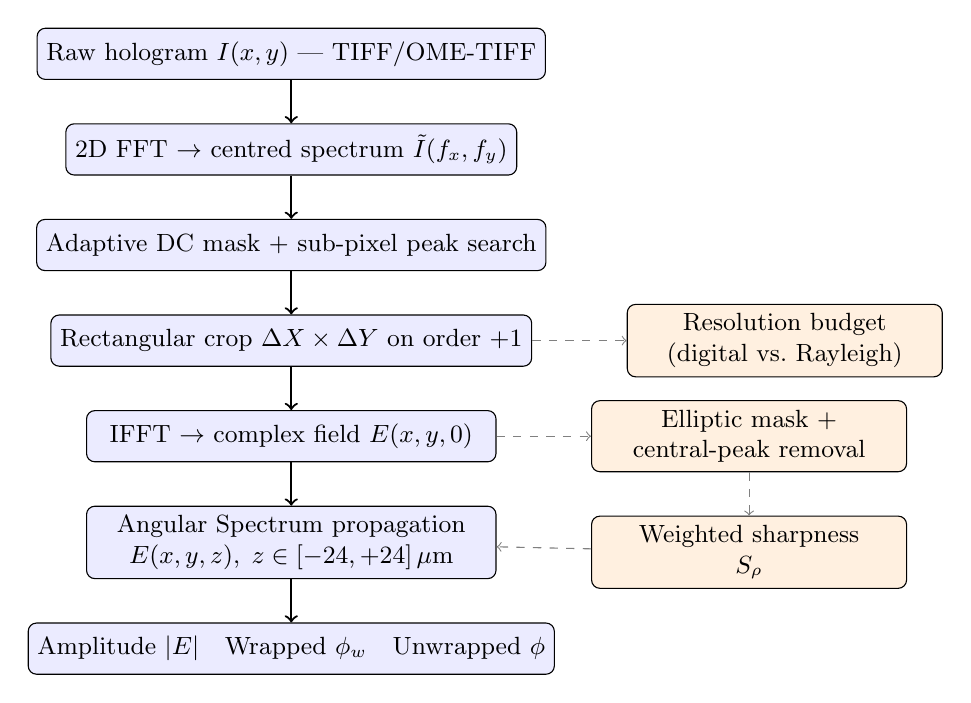
\begin{tikzpicture}[
    node distance   = 0.55cm and 1.2cm,
    box/.style      = {draw, rounded corners=3pt, fill=blue!8,
                       minimum width=5.2cm, minimum height=0.65cm,
                       font=\small, align=center},
    side/.style     = {draw, rounded corners=3pt, fill=orange!12,
                       minimum width=4.0cm, minimum height=0.65cm,
                       font=\small, align=center},
    arr/.style      = {->, thick},
    sarr/.style     = {->, dashed, gray}
]

\node[box] (load)   {Raw hologram $I(x,y)$ — TIFF/OME-TIFF};
\node[box, below=of load]  (fft)    {2D FFT $\to$ centred spectrum $\tilde{I}(f_x,f_y)$};
\node[box, below=of fft]   (gate)   {Adaptive DC mask + sub-pixel peak search};
\node[box, below=of gate]  (crop)   {Rectangular crop $\Delta X \times \Delta Y$ on order $+1$};
\node[box, below=of crop]  (ifft)   {IFFT $\to$ complex field $E(x,y,0)$};

\node[side, right=of crop]  (rescheck) {Resolution budget\\(digital vs.\ Rayleigh)};
\node[side, right=of ifft]  (mask)     {Elliptic mask +\\central-peak removal};
\node[side, below=of mask]  (sharp)    {Weighted sharpness\\$S_\rho$};

\node[box, below=of ifft]  (asm)    {Angular Spectrum propagation\\$E(x,y,z),\; z\in[-24,+24]\,\mu\text{m}$};
\node[box, below=of asm]   (maps)   {Amplitude $|E|$\quad Wrapped $\phi_w$\quad Unwrapped $\phi$};

\draw[arr] (load)  -- (fft);
\draw[arr] (fft)   -- (gate);
\draw[arr] (gate)  -- (crop);
\draw[arr] (crop)  -- (ifft);
\draw[arr] (ifft)  -- (asm);
\draw[arr] (asm)   -- (maps);

\draw[sarr] (crop)  -- (rescheck);
\draw[sarr] (ifft)  -- (mask);
\draw[sarr] (mask)  -- (sharp);
\draw[sarr] (sharp) -- (asm);

\end{tikzpicture}
\caption{Schematic of the digital holographic reconstruction pipeline.
         Solid arrows indicate the main data flow; dashed arrows indicate
         diagnostic/optional branches.}
\label{fig:pipeline}
\end{figure}



\input{Sections/Conclusions}

% --- INSERIMENTO PDF ESTERNO ---
% Se vuoi inserire un file PDF qui, decommenta la riga sotto:
% \includepdf[pages=-]{NomeDelTuoFile.pdf}

\newpage
% --- BIBLIOGRAFIA ---
\nocite{*} % Mostra tutti i riferimenti nel file .bib anche se non citati

\printbibheading[title={References}] % Aggiunge un titolo alla sezione bibliografia
\end{document}